\documentclass[a4paper,ngerman,11pt,bibliography=totoc]{scrartcl}


\usepackage[utf8]{inputenc}

\usepackage[ngerman]{babel}

\usepackage{amsmath, amsthm, amssymb, stmaryrd, color, graphicx, mathtools, mathrsfs}
\usepackage{setspace}
\usepackage{bussproofs}
\usepackage{array}
\usepackage{booktabs}
\usepackage{comment}
\usepackage{textcomp}
\usepackage{stmaryrd}

\usepackage{tikz}
\usetikzlibrary{shapes,arrows}
% Für kommutative Diagramme
\usepackage{tikz-cd}
% Vermeidet Konflikte mit babel ngerman (speziell bei Verwendung der \arrowvert[r, "Text"]-Notation)
\usetikzlibrary{babel}

\usepackage[protrusion=true,expansion=true]{microtype}

\usepackage{lmodern}
\usepackage{tabto}

\usepackage[backend=bibtex,style=alphabetic]{biblatex}
\usepackage[babel]{csquotes}
\bibliography{literatur}

% sidewaystable
\usepackage{rotating}

\usepackage{titling}

\usepackage[all]{xy}

% Automatische Referenzen mit Namen
\usepackage[colorlinks=true, linkcolor=blue, urlcolor=blue, citecolor=blue]{hyperref}
\usepackage{cleveref}			% Referenzen mit Name

\usepackage{icomma}				% Korrektes Typesetting von Kommazahlen

\usepackage[font={small,it}]{caption} % Kleinere Captions

% Für \Set{ ... | ... }
\usepackage{braket}
% Für fette Symbole in Math-Umgebung (\bm)
\usepackage{bm}

% Symbole...
\usepackage{fontawesome}
\pdfmapfile{+fontawesome.map}

% Transparente Farben
\usepackage{transparent}

%\usepackage{algorithm}
%\usepackage{algpseudocode}
%\algrenewcommand{\algorithmiccomment}[1]{\hskip3em$\slash\slash$ #1}
%\newcommand{\LineFor}[2]{\State\algorithmicfor\ {#1}\ \algorithmicdo\ {#2} \algorithmicend\ \algorithmicfor}
%
%\usepackage{listings}			% Anzeige von Sourcecode

\setlength\parskip{\medskipamount}
\setlength\parindent{0pt}

\theoremstyle{definition}
\newtheorem{defn}{Definition}[section]
\newtheorem{axiom}[defn]{Axiom}
\newtheorem{bsp}[defn]{Beispiel}

\theoremstyle{plain}

\newtheorem{prop}[defn]{Proposition}
\newtheorem{lemma}[defn]{Lemma}
\newtheorem{kor}[defn]{Korollar}
\newtheorem{satz}[defn]{Satz}

\theoremstyle{remark}
\newtheorem{erin}[defn]{Erinnerung}
\newtheorem{bem}[defn]{Bemerkung}
\newtheorem{beob}[defn]{Beobachtung}
\newtheorem{notation}[defn]{Notation}

\clubpenalty=10000
\widowpenalty=10000
\displaywidowpenalty=10000

\newcommand{\IZ}{\mathbb{Z}}
\newcommand{\IQ}{\mathbb{Q}}
\newcommand{\IR}{\mathbb{R}}
\newcommand{\IC}{\mathbb{C}}
\newcommand{\IN}{\mathbb{N}}
\newcommand{\INo}{\IN_0}
\newcommand{\INs}{\IN^\ast}
\newcommand{\Ic}{\mathcal{I}}
\newcommand{\Jc}{\mathcal{J}}
\newcommand{\Hc}{\mathcal{H}}
\newcommand{\Tc}{\mathcal{T}}
\newcommand{\Sc}{\mathcal{S}}
\newcommand{\Oc}{\mathcal{O}}
\newcommand{\Pc}{\mathcal{P}}

\newcommand{\PSet}{\Pc}		% Potenzmenge

\newcommand{\ceil}[1]{\left\lceil#1\right\rceil}
\newcommand{\abs}[1]{\left|#1\right|}

\newcommand{\from}{\leftarrow}

\newcommand{\id}{\mathrm{id}}

\newcommand{\setMid}{\,\middle|\,}

% Supresses qed-symbol in current environment
\newcommand{\noqed}{\let\qed\relax}

\newcommand{\symDiff}{\triangle}


%draft-options:
\definecolor{darkgreen}{rgb}{0,0.6,0.35}
\usepackage[ngerman, textsize=small, textwidth=4.5cm, color=darkgreen]{todonotes}
\usepackage[left=1cm, right=5cm]{geometry}


% Nur für dieses Dokument %%%%%%%%%%%%%%%%%%%%%%%%%%%%%%%%%%%%%%

\setcounter{tocdepth}{3}


\usepackage{tabu}
\usepackage{tabularx}


\newcommand{\dIff}{\mathbin{~\mathop:\!\!\iff}}

% Ordnungsrelation auf dem Kostenraum
\newcommand{\cordleq}{\preccurlyeq}
\newcommand{\cordgeq}{\succcurlyeq}
\newcommand{\cordle}{\prec}
\newcommand{\cordge}{\succ}

\newcommand{\PfadAend}{\delta}
\newcommand{\invPf}[1]{\overset{\leftarrow}{#1}}
\newcommand{\Pfadkomp}{\cdot}

\newcommand{\SVord}{\ensuremath \prec_\uparrow}
\newcommand{\NVrel}{\approx}
\newcommand{\XmodNV}{X/{\NVrel}}
\newcommand{\VerbRel}{\ensuremath <_\uparrow}
\newcommand{\BAord}{\ensuremath \prec^\ast}
\newcommand{\BArel}{\approx^\ast}
\newcommand{\XmodBA}{X/{\BArel}}

% Sammelbegriff für alle Potentialbegriffe
\newcommand{\sPot}{\_-Potential}

% Für Spiele
\newcommand{\Epsilon}{\mathrm{E}}
\newcommand{\Kappa}{\mathrm{K}}
\newcommand{\Dummy}{\mathrm{D}}

% Spieler (aus Menge I)
\newcommand{\ia}{{i'}}
\newcommand{\ib}{{\hat{\imath}}}

% DOCUMENT %%%%%%%%%%%%%%%%%%%%%%%%%%%%%%%%%%%%%%%%%%%%%%%%%%%%%

\begin{document}
	
% Spezielle Silbentrennung:
\hyphenation{Ko-or-di-na-tion Ko-or-di-na-tions-spie-len Ko-or-di-na-tions-spiels Be-o-bach-tung Po-ten-tial-funk-ti-on}	
	
	
% Titelseite:

\author{Lukas Graf}
\date{Letzte Aktualisierung: \today}

\selectlanguage{ngerman}
\thispagestyle{empty}


\begin{titlepage}\center
	\textsc{\LARGE Universität Augsburg}\\[1cm]
	
	\textsc{\Large Institut für Mathematik}\\[1.5cm]
	
	% Title
	{\Large Masterarbeit \\[1cm]}
	{\huge \todo[inline]{Insert Title}}

	\vfill
	
	% Author and supervisor
	\begin{minipage}{0.4\textwidth}
		\begin{flushleft} \large
			\emph{von:}\\
			Lukas \textsc{Graf}
		\end{flushleft}
	\end{minipage}
	\begin{minipage}{0.4\textwidth}
		\begin{flushright} \large
			\emph{Betreut von:} \\
			Prof. Dr. Tobias \textsc{Harks}
		\end{flushright}
	\end{minipage}
	
\end{titlepage}

% CONTENT %%%%%%%%%%%%%%%%%%%%%%%%%%%%%%%%%%%%%%%%%%%

\tableofcontents

\phantomsection
\addcontentsline{toc}{section}{Einleitung}
\section*{Einleitung}

Nicht-kooperative Spiele in strategischer Form sind eine einfache, aber zugleich mächtige Art und Weise eine Vielzahl von Spielen oder spielartigen Situationen mathematisch zu beschreiben. Ein Spiel wird hierbei dadurch angegeben, dass jeder Spieler eine Menge ihm zur Verfügung stehender Strategien sowie eine eigene Kostenfunktion (oder Auszahlungsfunktion) auf dem Produktraum aller spielerspezifischen Strategieräume hat. \glqq Gespielt\grqq{} wird ein solches Spiel, indem jeder Spieler eine seiner Strategien auswählt (ohne dabei die Wahlen der anderen Spieler zu kennen). Hat jeder Spieler dies getan, so legt die Gesamtheit aller gewählten Strategien das Ergebnis des Spiels fest, welches dann jeder Spieler mit Hilfe seiner Kostenfunktion für sich bewerten kann.

Von besonderem Interesse bei der Analyse derartiger Spiele sind Nash-Gleichgewichte: Spielsituationen, in denen keiner der Spieler (aus rein egoistischer Sicht) ein Interesse daran hat einseitig seine gewählte Strategie zu ändern - also Situationen, in denen jede alleinige Strategieänderung eines Spielers zu einem schlechteren oder höchstens genauso guten Ergebnis für diesen Spieler führt. Die Fragen, welche Spiele solch ein Nash-Gleichgewicht besitzen, welche Eigenschaften dieses dann besitzt und wie man es finden kann, gehören zu den zentralen Fragestellungen der Spieltheorie.

Eine Klasse von anschaulichen (endlichen) Spielen, die zudem immer wenigstens ein Nash-Gleichgewicht besitzen, fand \citeauthor{RosenthalPotential} mit den sogenannten Auslastungsspielen. Dabei handelt es sich um Spiele, in denen jeder Spieler festlegt, welche Teilmenge einer gemeinsamen Menge von Ressourcen er nutzt, wobei deren Kosten davon abhängen, wie viele Spieler die jeweilige Ressource nutzen. Im Beweis der Existenz eines solchen Gleichgewichtes nutzte \citeauthor{RosenthalPotential} eine Art gemeinsame Kostenfunktion für alle Spieler, eine sogenannte Potentialfunktion. Die durch diese Potentialfunktion beschriebenen Kosten sind dabei auf geeignete Weise mit den ursprünglichen spielerspezifischen Kosten verträglich, sodass ein Minimum der Potentialfunktion automatisch auch ein Nash-Gleichgewicht des eigentlichen Spiels ist.

Später bewiesen \citeauthor{MonShap}, dass sich umgekehrt auch jedes Spiel, welches eine derartige Potentialfunktion besitzt, als Auslastungsspiel darstellen lässt, es also ein Auslastungsspiel gibt, welches äquivalent zu dem Potentialspiel ist. Zudem definierten sie weitere, allgemeinere Potentialbegriffe, welche ebenfalls die Suche von Nash-Gleichgewichten erleichtern, aber dabei auch für Spiele anwendbar sind, welche nicht durch \citeauthor{RosenthalPotential}s Auslastungsspiele darstellbar sind. 

Beide beschriebenen Sätze nutzen als zentrales Element spezielle Arten von Beziehungen zwischen zwei Spielen (einmal zwischen einem Spiel und dem durch die Potentialfunktion beschriebenen alternativen Spiel und einmal zwischen dem Potentialspiel und dem es darstellenden Auslastungsspiel). Im Rahmen dieser Arbeit wollen wir diese Idee einer Beziehung zwischen zwei Spielen, die gewisse Eigenschaften wie etwa Nash-Gleichgewichte erhält, formalisieren und näher untersuchen. Außerdem werden wir versuchen weitere derartige Beziehungen zwischen verschiedenen Klassen von Spielen zu finden.

Nachdem wir in \Cref{sec:Grundlagen} einige Grundbegriffe der Spieltheorie definiert haben, werden wir uns zunächst in \Cref{sec:Potentiale} dem Konzept von Potentialfunktionen für Spiele zuwenden. Wir werden eine ganze Reihe derartiger Potentiale kennenlernen und jeweils notwendige und hinreichende Bedingungen dafür zeigen, dass ein Spiel ein entsprechendes Potential besitzt. Im folgenden \Cref{sec:Morphismen} werden wir verschiedene Arten von Morphismen zwischen Spielen definieren, die dann Isomorphien induzieren, die wir nutzen können um die besagten Beziehungen zwischen verschiedenen Spielen beschreiben zu können. In \Cref{sec:Auslastungsspiele} schließlich werden wir diese (Iso-)Morphismen nutzen, um einige Zusammenhänge zwischen unterschiedlichen Klassen von Auslastungs- und Potentialspielen zu formulieren und zu beweisen.

Wir werden dabei immer versuchen die verschiedenen Sätze möglichst allgemein zu halten und insbesondere - soweit dies möglich ist - auch über unendliche statt, wie in der Literatur meist üblich, nur über endliche Spiele sprechen.

\listoftodos

\section{Grundlagen}\label{sec:Grundlagen}

\begin{defn}
	Ein \emph{Spiel $\Gamma$ in strategischer Form} ist ein Tupel $(I, X = (X_i)_{i \in I}, (K_i)_{i\in I}, (c_i)_{i\in I})$. Dabei ist
	\begin{itemize}
		\item $I$ die Menge der Spieler,
		\item $X_i$ die Menge der (reinen) Strategien von Spieler $i$,
		\item $(K_i, \cordleq)$, eine total geordnete Menge, der Kostenraum von Spieler $i$ und
		\item $c_i: X \to K_i$ die Kostenfunktion von Spieler $i$.
	\end{itemize}
	Das eigentliche Spiel besteht nun daraus, dass jeder Spieler versucht durch die Wahl seiner Strategie seine Kosten zu minimieren.
\end{defn}

\begin{beob}
	Klassische Kostenminimierungsspiele erhält man durch Wahl von $(\IR_{\geq 0}, \leq)$ als Kostenraum für alle Spieler, Nutzenmaximierungsspiele durch Wahl von $(\IR, \geq)$ als \glqq Kosten\grqq raum.
\end{beob}

\begin{notation}
	Zu einem festen Spieler $i$ bezeichne $X_{-i} := \prod_{j \in I\backslash\{i\}} X_j$ das Produkt aller Strategieräume außer dem von Spieler $i$. Zu jedem Strategieprofil\todo{Sollte der Begriff Strategieprofil eigens definiert werden?}{} $x \in X$ bezeichne dann $x_{-i}$ die Projektion dieses Profils auf den Raum $X_{-i}$ und $x_i$ die Projektion auf $X_i$ (also die von Spieler $i$ gewählte Strategie). Wir schreiben dann auch $(x_i, x_{-i})$ für das Strategieprofil $x$.
\end{notation}

\begin{defn}
	Ein Strategieprofil $x \in X$ ist ein \emph{Nash-Gleichgewicht}, wenn für jeden Spieler $i \in I$ und jede seiner Strategien $\hat{x}_i$ gilt:
		\[c_i(\hat{x}_i, x_{-i}) \cordgeq c_i(x)\]
	Ein Nash-Gleichgewicht ist also ein Strategieprofil, aus dem heraus kein Spieler einen Anreiz für einen einseitigen Strategiewechsel hat.	
\end{defn}

Aus \cite{MonShap}:

\begin{defn}
	Eine Folge von Strategieprofilen $x^0, x^1, x^2, \dots$ ist ein \emph{Verbesserungspfad}, wenn folgende beiden Eigenschaften erfüllt sind:
	\begin{enumerate}
		\item Für jede Stelle $n$ gibt es einen Spieler $i(n) \in I$, sodass das Profil $x^{n+1}$ aus $x^n$ durch alleinige Abweichung dieses Spielers entsteht, d.h. $x^{n+1} = (x^{n+1}_{i(n)}, x^n_{-i(n)})$
		\item Der abweichende Spieler $i(n)$ verbessert sich, d.h. $u_{i(n)}(x^{n+1}) \cordle u_{i(n)}(x^n)$.
	\end{enumerate}
\end{defn}

\begin{defn}
	Ein Spiel $\Gamma$ hat die \emph{finite improvement property (FIP)}, wenn jeder Verbesserungspfad endlich ist.
\end{defn}

\begin{beob}
	Jedes Ende eines maximalen Verbesserungspfades ist ein Nash-Gleichgewicht. Denn wäre dem nicht so, dann gäbe es wenigstens einen Spieler, der sich durch Abweichen noch verbessern kann - was zu einer Verlängerung des Verbesserungspfades führen würde. Ein Spiel mit FIP besitzt daher wenigstens ein Nash-Gleichgewicht.
\end{beob}
\section{Potentiale}\label{sec:Potentiale}

\subsection{Definitionen}

\begin{defn}
	Eine Funktion $P: X \to \IR$ heißt\todo{Verallgemeinern? (total geordnete Menge $K$ statt $\IR$?)}
	\begin{itemize}
		\item \emph{Beste Antwort-Potential}, wenn für jeden Spieler $i$ und alle Strategieprofile $x_{-i} \in X_{-i}$ gilt:
			\[\arg \min_{x_i \in X_i}c_i(x) = \arg \min_{x_i \in X_i} P(x)\]
		\item \emph{verallgemeinertes ordinales Potential}, wenn für jeden Spieler $i$ und alle Strategieprofile $x_{-i} \in X_{-i}$ sowie $x_i, \hat{x}_i \in X_i$ gilt:
			\[c_i(x_i,x_{-i}) > c_i(\hat{x}_i, x_{-i}) \implies P(x_i,x_{-i}) > P(\hat{x}_i, x_{-i})\]
		\item \emph{ordinales Potential}, wenn für jeden Spieler $i$ und alle Strategieprofile $x_{-i} \in X_{-i}$ sowie $x_i, \hat{x}_i \in X_i$ gilt:
			\[c_i(x_i,x_{-i}) > c_i(\hat{x}_i, x_{-i}) \iff P(x_i,x_{-i}) > P(\hat{x}_i, x_{-i})\]
		\item \emph{skaliertes Potential}, wenn es streng monotone Funktionen $f_i: \IR \to \IR$ gibt, die $0$ auf $0$ abbilden, sodass für jeden Spieler $i$ und alle Strategieprofile $x_{-i} \in X_{-i}$ sowie $x_i, \hat{x}_i \in X_i$ gilt:
			\[c_i(x_i,x_{-i}) - c_i(\hat{x}_i, x_{-i}) = f_i(P(x_i,x_{-i}) - P(\hat{x}_i, x_{-i}))\]
		\item \emph{gewichtetes Potential}, wenn es einen Gewichtsvektor $(w_i)_{i\in I} \in \IR_{>0}^I$ gibt, sodass für jeden Spieler $i$ und alle Strategieprofile $x_{-i} \in X_{-i}$ sowie $x_i, \hat{x}_i \in X_i$ gilt:
			\[c_i(x_i,x_{-i}) - c_i(\hat{x}_i, x_{-i}) = w_i\cdot(P(x_i,x_{-i}) - P(\hat{x}_i, x_{-i}))\]
		\item \emph{exaktes Potential}, wenn für jeden Spieler $i$ und alle Strategieprofile $x_{-i} \in X_{-i}$ sowie $x_i, \hat{x}_i \in X_i$ gilt:
			\[c_i(x_i,x_{-i}) - c_i(\hat{x}_i, x_{-i}) = P(x_i,x_{-i}) - P(\hat{x}_i, x_{-i})\]
	\end{itemize}
\end{defn}\todo{Kann man diese Definition irgendwie kompakter/übersichtlicher machen?}

Exakte, gewichtete, ordinale und verallgemeinerte ordinale Potentiale wurden erstmals in \cite{MonShap} definiert, beste Antwort-Potentiale erstmals in \cite{BestRespPot}.

\subsection{Anschauung}

In einem gewissem Sinne definiert jedes Potential ein alternatives Spiel mit gleichem Strategieraum, aber einer anderen, für alle Spieler einheitlichen Kostenfunktion (nämlich der Potentialfunktion). In einem solchen Spiel ist es nun viel einfacher beispielsweise Gleichgewichts- oder Optimalitätspunkte zu finden (da hierzu nur eine einzige Funktion betrachtet werden muss). Eigenschaften, die beim Übergang zurück zum ursprünglichen Spiel erhalten bleiben, kann man dann in dem einfacheren Spiel überprüfen. Diesen Übergang werden wir später mit Hilfe von (Iso-)Morphismen formal fassen (siehe \Cref{sec:Morphismen}).

Hier wollen wir nun noch kurz darauf eingehen, wie sich die verschiedenen Potentialbegriffe anschaulich voneinander unterscheiden. Wir betrachten dazu (endliche) 2-Personenspiele. Deren Strategieraum kann man dann als Gitternetz in der Ebene auffassen, wobei jede Strategie von Spieler 1 einer senkrechten und jede Strategie von Spieler 2 einer waagerechten Gitterlinie entspricht. Kreuzungspunkte von zwei Gerade entsprechen dann gerade vollständige Strategieprofilen. Kostenfunktionen (ebenso wie Potentiale) sind dann \glqq Reliefkarten\grqq{}, deren Höhe den jeweiligen Kosten entspricht. 

\begin{figure}[h]\centering
	\includegraphics[width=.3\textwidth]{../Bilder/exaktesPotentialSp1.pdf}
	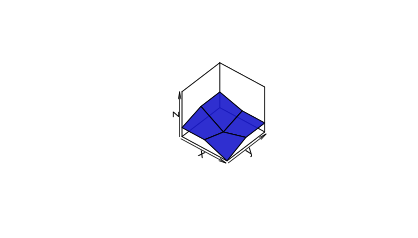
\includegraphics[width=.3\textwidth]{../Bilder/exaktesPotentialSp2.pdf}
	\includegraphics[width=.3\textwidth]{../Bilder/exaktesPotential.pdf}
	\caption{Ein 2-Personenspiel mit exaktem Potential (grau): Spieler 1: rot, Spieler 2: blau}
\end{figure}

Ein exaktes Potential entspricht in diesem Bild einer gemeinsamen Reliefkarte für beide Spieler, die - im Falle eines exakten Potentials - \glqq scheibenweise\grqq{} bis auf eine additive Konstante mit der eigentlichen Kostenfunktion übereinstimmt. Anders formuliert: Wird die Strategie eines Spieler festgehalten, so kann der andere Spieler seine Kostenveränderungen bei der Wahl der verschiedenen ihm zur Verfügung stehenden Strategien auch anhand der Potentialfunktion ablesen. 

Geht man nun über zu einem gewichteten Potential, so lesen die beiden Spieler das Potential sozusagen in verschiedenen Einheiten\todo{eigentlich müssen verchiedene Einheiten nicht zwangsläufig proportional zueinander sein - für Längeneinheiten sollte es typischerweise aber stimmen}. Das heißt die Kostenveränderungen eines Spielers sind nur noch proportional zu den Potentialänderungen. Ein skaliertes Potential zeigt jedem Spieler noch an, welche der Kostenveränderungen eher groß und welche klein sind. Ordinale Potentiale zeigen nur noch die Richtung der Kostenveränderung an (\glqq wird teurer\grqq / \glqq wird billiger\grqq / \glqq Kosten bleiben konstant\grqq) und verallgemeinerte ordinale Potentiale zeigen nur noch echte Steigungen korrekt an. Beste-Antwort-Potentiale schließlich zeigen immer die beste Antwort an.


\todo[inline]{Zusammenhänge (evtl. schon nächstes Kapitel?)}

Eine Beobachtung aus \cite{CharExGewPotinWCG}:

\begin{beob}\label{beob:ZshExGewPot}
	Ein Spiel $\Gamma = (I, (X_i)_{i \in I}, (c_i)_{i \in I})$ besitzt genau dann ein gewichtetes Potential (mit Gewichtsvektor $(w_i)_{i \in I}$), wenn $\Gamma' := (I, (X_i)_{i \in I}, (w_i \cdot c_i)_{i \in I})$ ein exaktes Potential besitzt.
\end{beob}

Folgt auch aus einer allgemeineren Beobachtung in \Cref{sec:Morphismen}.

\subsection{Erste Sätze}

Zu einem gegebenen Strategieprofil $x \in X$ sei dessen \emph{Nachbarschaft} die Menge aller durch höchstens eine Abweichung erreichbarer Strategieprofile, d.h. die Menge $\{(\hat{x}_i, x_{-i}) | i \in N, \hat{x}_i \in X_i\}$. Wir nennen $x$ dann ein \emph{lokales Minimum} einer Funktion $f: X \to \IR$, wenn es ein Minimum innerhalb seiner Nachbarschaft ist.

\begin{satz}\label{satz:lokMinNG}
	Sei $\Gamma$ ein Spiel mit einem verallgemeinerten ordinalen Potential $P$. Dann ist jedes lokale Minimum von $P$ ein Nash-Gleichgewicht von $\Gamma$. Ist $P$ sogar ein ordinales Potential, so gilt auch die umgekehrte Richtung.
\end{satz}

\todo[inline]{Diese Sätze hier evtl. nur erwähnen und erst später (nach der Definition von Morphismen) formalisieren (und beweisen)}

Dieser Satz zeigt also, dass man Nash-Gleichgewichte allein durch Betrachten einer Potentialfunktion finden kann. Daraus  folgt direkt die Existenz von Nash-Gleichgewichten in einer Vielzahl von Potentialspielen:

\begin{kor}
	Sei $\Gamma$ ein Spiel mit einem kompakten Strategieraum und einer stetigen verallgemeinerten ordinalen Potentialfunktion. Dann hat $\Gamma$ wenigstens ein Nash-Gleichgewicht.
\end{kor}

Insbesondere also haben endliche Potentialspiele immer ein Nashgleichgewicht. \Cref{satz:lokMinNG} folgt mit Hilfe von \Cref{kor:ExVerbPfadExNG} direkt aus dem folgenden Satz\todo{Streng genommen nicht wirklich, da das Korollar nur für Spiele gilt!?}:

\begin{satz}
	Sei $\Gamma$ ein Spiel mit einem verallgemeinerten ordinalen Potential $P$. Dann ist jeder Verbesserungspfad in $\Gamma$ auch ein Verbesserungspfad bezüglich $P$. Ist $P$ sogar ein ordinales Potential, so gilt auch die umgekehrte Richtung.
\end{satz}

\begin{proof}.
	
	\todo[inline]{Beweis}	
\end{proof}

\todo[inline]{Was kann man über Beste-Antwort-Potentiale sagen (vermtl. Zusammenhang zu Beste-Antwort-Pfade?)}

Für Spiele mit unendlicher Spielermenge erweist es sich als hilfreiche Beobachtung, dass wir Potentiale pfadzusammenhangskomponentenweise definieren können:

\begin{beob}\label{beob:KompWeisePotentiale}
	Sei $\Gamma$ ein beliebiges Spiel und $P: X \to \IR$ eine Funktion. Erfüllt $P$ dann die Bedingung eines exakten/gewichteten/skalierten/ordinalen/verallgemeinerten ordinalen Potentials für jede (maximale) Pfadzusammenhangskomponente, so ist $P$ ein entsprechendes Potential für ganz $\Gamma$.
\end{beob}

\begin{proof}
	Dies folgt direkt aus dem Umstand, dass die definierende Eigenschaft für alle aufgezählten Potentiale immer nur entlang eines Pfades (der Länge $1$) und damit innerhalb einer Zusammenhangskomponente geprüft werden muss.
\end{proof}

\subsection{Charakterisierungen der Potentiale}

\begin{satz}\label{satz:CharExPot}
	Ein Spiel besitzt genau dann ein exaktes Potential, wenn alle 4-Zykel im Strategieraum eine Gesamtänderung von $0$ haben.
\end{satz}

\begin{proof}
	Wir folgen dem Beweis aus \cite[Anhang A]{MonShap}. Dort wird der Satz nur für $N$-Personenspiele gezeigt, mit \Cref{beob:KompWeisePotentiale} überträgt sich dieser Beweis aber direkt auch auf allgemeine Spiele.
	
	Sei zunächst $\gamma \coloneqq (x^0, x^1, x^2, x^3, x^4)$ ein beliebiger 4-Zykel in einem Spiel mit Potential $P$. Dann gilt für die Gesamtänderung:
		\[\delta(\gamma) = \sum_{i=0}^3 \left(c_{i(k)}(x^{k+1}) - c_{i(k)}(x^k)\right) = \sum_{k=0}^{3} \left(P(x^{k+1}) - P(x^k)\right) = P(x^4) - P(x^0) = 0^{}\]
		
	Ist umgekehrt $\Gamma$ ein Spiel, in dem für alle 4-Zykel $\gamma$ gilt $\PfadAend(\gamma) = 0$, $x$ ein beliebiges, aber festes Strategieprofil in $\Gamma$ und $Y_x$ dessen Pfadzusammenhangskomponente. Dann definiere wie folgt eine Funktion $P_x$ auf $Y_x$:
		\[P: Y_x \to \IR: y \mapsto \PfadAend(\gamma), \,\gamma \text{ beliebiger Pfad von } x \text{ nach } y \]
	Damit diese Funktion tatsächlich wohldefiniert ist, muss für je zwei Pfade $\gamma$ und $\gamma'$ von $\hat{x}$ nach $x$ gelten, dass die jeweiligen Gesamtänderungen gleich sind, d.h. $\PfadAend(\gamma) = \PfadAend(\gamma')$. Dies ist äquivalent dazu, dass der Zykel, den man durch Verknüpfen der beiden Pfade $\gamma$ und $\overset{\leftarrow}{\gamma'}$ erhält eine Gesamtänderung von $0$ hat. Dazu zeigen wir nun mittels Induktion über deren Länge, dass für alle Zykel $\mu$ gilt $\PfadAend(\mu) = 0$:
	\begin{description}
		\item[IA ($\abs{\mu}=4$)] D.h. $\mu$ ist ein 4-Zykel und damit $\PfadAend(\mu) = 0$ nach Voraussetzung.
		\item[IS ($\abs{\mu}\eqqcolon n$)] Vorausgesetzt es gibt einen Pfad $\mu' = (x'^0, \dots, x'^n)$ gleicher Länge und Gesamtänderung wie $\mu$, sodass in den ersten beiden Schritten der gleiche Spieler seine Strategie wechselt, d.h. $i(0)=i(1)$. Dann erhält man durch Weglassen des ersten Schrittes einen \emph{kürzeren} Pfad $\mu'' \coloneqq (x'^0, x'^2, \dots, x'^n)$ mit gleicher Gesamtänderung, welche dann nach Induktion bereits $0$ ist. Indiesem Fall haben wir dann wie gewünscht $\PfadAend(\mu) = \PfadAend(\mu') = \PfadAend(\mu'') = 0$.
		
		Die Existenz eines solchen Pfades $\mu'$ zeigen wir nun mittels Induktion über $k \coloneqq min\left\{1 \leq l < n \setMid i(l) = i(0)\right\}$. Ein solches $k$ existiert immer, da Spieler $i(0)$ bereits im ersten Schritt seine Strategie wechselt und dies daher im Verlauf des Zykels noch mindestens ein weiteres Mal tun muss.
		\begin{description}
			\item[IA ($k=1$)] Dann gilt bereits $i(0)=i(1)$ und wir sind fertig mit $\mu' \coloneqq \mu$.
			\item[IS ($k-1\to k$)] Wir ändern $\mu$ so ab, dass Spieler $i(0)$ bereits im $(k-1)$-ten Schritt der abweichende Spieler ist. Dann sind wir fertig nach Induktionsvoraussetzung. Dazu ersetzen wir in $\mu$ das Strategieprofil $x^k$ durch $(x^{k-1}_{-i(0)}, x^{k+1}_{i(0)})$, sodass also Spieler $i(0)$ bereits einen Schritt früher (im $(k-1)$-ten) seine Strategie wechselt und der Spieler, der dies zuvor in diesem Schritt getan hat, einen Schritt später.
			
			Bei dieser Anpassung bleibt die Gesamtänderung des Pfades $\mu$ gleich, denn wir ersetzen lediglich ein Pfadstück der Länge $2$ durch ein anderes Pfadstück der Länge $2$. Und da sich diese beiden Pfade zu einem 4-Zykel zusammensetzen lassen, haben diese nach Voraussetzung die gleiche Gesamtänderung.
			
			Auf dieses abgeänderte $\mu$ können wir nun die Induktionsvoraussetzung anwenden und erhalten dadurch einen neuen Pfad $\mu'$ mit den gewünschten Eigenschaften.
		\end{description}
		Hiermit können wir auch den Induktionsschritt der äußeren Induktion und damit den Nachweis der Wohldefiniertheit von $P$ abschließen. 
	\end{description}	
	Wählen wir nun für jede maximale Pfadzusammenhangskomponente ein einziges $x$ in dieser und definieren wie oben eine Funktion $P_x$, so lassen sich alle diese Funktionen zu einer Funktion $P$ auf ganz $X$ zusammensetzen. Nach Definition erfüllt diese auf jeder Pfadzusammenhangskomponente die Bedingung eines exakten Potentials. Also ist nach \Cref{beob:KompWeisePotentiale} $P$ ein exaktes Potential auf $X$.
\end{proof}

\begin{satz}\label{satz:CharGewPot}
	Ein Spiel besitzt genau dann ein gewichtetes Potential, wenn ... \todo{analoge Bedingung zu exaktem Potential (vgl. \cite[Kapitel 3.2]{CharExGewPotinWCG})}
\end{satz}

\begin{proof}.
	
	\todo[inline]{mit \Cref{beob:ZshExGewPot}?}
\end{proof}

\todo[inline]{Charakterisierung der Existenz eines skalierten Potentials?}

\begin{defn}
	Eine Menge $X$ mit einer strikten Partialordnung $\prec$ (irreflexiv und transitiv) heißt \emph{reell geordnet}\footnote{\citeauthor{CharExOrdPot} bezeichnen solche Mengen in \cite{CharExOrdPot} als \glqq properly ordered\grqq}, wenn es eine strikt monotone Abbildung von $X$ in die reellen Zahlen gib, also $f: X \to \IR$ mit $x \prec x' \implies f(x) < f(x')$.
\end{defn}

Wir definieren nun eine Äquivalenzrelation auf dem Strategieraum:\todo{evtl. schon im Grundlagenkapitel gemeinsam mit Pfadzusammenhangskomponenten?}
	\[x \NVrel y \dIff \text{ es gibt einen nicht-Verschlechterungspfad von $x$ nach $y$ und umgekehrt}\]
Auf dem dadurch erzeugten Raum von Äquivalenzklassen $\XmodNV \coloneqq \left\lbrace[x] \mid x \in X\right\rbrace$ erhält man eine transitive Ordnung
	\[[x] \SVord [y] \dIff \text{Es gibt einen schwachen Verbesserungspfad von $y$ nach $x$}\]
Sowohl Wohldefiniertheit als auch Transitivität dieser Relation ergeben sich aus der Beobachtung, dass die Verknüpfung eines nicht-Verschlechterungspfades mit einem schwachen Verbesserungspfad wieder einen schwachen Verbesserungspfad ergibt.

Damit zeigen \citeauthor{CharExOrdPot} in \cite[Theorem 3.1]{CharExOrdPot} folgende Charakterisierung der Existenz von ordinalen Potentialen:

\begin{satz}\label{satz:CharOrdPot}
	Ein Spiel besitzt genau dann ein ordinales Potential, wenn es keine schwachen Verbesserungszykel enthält und $(\XmodNV, \SVord)$ reell geordnet ist.
\end{satz}

\begin{proof}
	Sei zunächst $P: X \to \IR$ ein ordinales Potential eines Spiels $\Gamma$. Dann gilt:
	\begin{enumerate}
		\item $\Gamma$ enthält keine schwachen Verbesserungszykel. Denn angenommen $\gamma = (x^0, \dots, x^n)$ wäre ein schwacher Verbesserungszykel in $\Gamma$, so gilt für alle $0 \leq k < n$: $c_{i(k)}(x^{k+1}) \cordleq c_{i(k)}(x^k)$ und für ein solches $k$ sogar $c_{i(k)}(x^{k+1}) \cordle c_{i(k)}(x^k)$. Da ferner $P$ ein ordinales Potential ist, folgt daraus:
			\[P(x^0) \leq P(x^1) \leq \dots \leq P(x^{k+1}) < P(x^k) \leq \dots \leq P(x^n) = P(x^0)\]
		Dies ist jedoch ein Widerspruch. Also kann es keinen solchen Verbesserungszykel geben.
		
		\item $\SVord$ ist eine strikte Partialordnung auf $\XmodNV$. Denn die Relation ist immer transitiv und in der Abwesenheit von schwachen Verbesserungszykeln zudem irreflexiv. Gäbe es nämlich en Strategieprofil mit $[x] \SVord [x]$, so gäbe es einen schwachen Verbesserungspfad von $x$ nach $x$, also einen schwachen Verbesserungszykel.
		
		\item $(\XmodNV, \SVord)$ ist reell geordnet. Definiere dazu die Abbildung $f: X/{\approx} \to \IR: [x] \mapsto P(x)$. Diese ist wohldefiniert, denn ist $y \in [x]$, so gibt es also nicht-Verschlechterungspfade von $x$ nach $y$ und umgekehrt. Zusammen bilden dieses einen nicht-Verschlechterungszykel und da es keine schwachen Verbesserungszykel in $\Gamma$ gibt, muss in die diesem Zykel (und damit bereits in den beiden Pfaden) in jedem Schritt Gleichheit gelten. Insbesondere folgt damit $P(x) = P(y)$.
		
		Ferner ist diese Abbildung streng monoton, denn gilt $[x] \SVord [y]$, so gibt es einen nicht-Verschlechterungspfad $\gamma$ von $y$ nach $x$, aber keinen in die umgekehrte Richtung. Insbesondere ist also $\overset{\leftarrow}{\gamma}$ kein nicht-Verschlechterungspfad, d.h. $\gamma$ ein schwacher Verbesserungspfad von $y$ nach $x$. Damit folgt analog zum ersten Punkt: $P(x) < P(y)$
	\end{enumerate}

	Ist umgekehrt $\Gamma$ ein Spiel ohne schwache Verbesserungszykel und $([X], \SVord)$ reell-geordnet mit Abbildung $f: [X] \to \IR$, so definiere $P: X \to \IR: x \mapsto f([x])$. Dies ist ein ordinales Potential, denn es gilt:
	\begin{enumerate}
		\item Gilt $c_i(x) > c_i(\hat{x}_i, x_{-i})$, so ist $(x, (\hat{x}_i, x_{-i}))$ ein schwacher Verbesserungspfad. Da es in $\Gamma$ keine schwachen Verbesserungszykel gibt, kann es also keinen nicht-Verschlechterungspfad in die andere Richtung geben und es gilt: $[x] \succ [(\hat{x}_i, x_{-i})]$. Daraus wiederum folgt $P(x) = f([x]) > f([(\hat{x}_i, x_{-i})]) = P(\hat{x}_i, x_{-i})$.
		\item Gilt $c_i(x) = c_i(\hat{x}_i, x_{-i})$, so sind sowohl $(x, (\hat{x}_i, x_{-i}))$ als auch $((\hat{x}_i, x_{-i}), x)$ nicht-Verschlechterungspfade, also $[x] = [(\hat{x}_i, x_{-i})]$ und damit $P(x) = f([x]) = f([(\hat{x}_i, x_{-i})]) = P(\hat{x}_i, x_{-i})$. \qedhere
	\end{enumerate}
\end{proof}

\begin{bem}
	Im Gegensatz zur Charakterisierung von exakten Potentialspielen in \Cref{satz:CharExPot} genügt es für die Existenz eines ordinalen Potentials nicht, nur Zykel der Länge 4 zu betrachten. \citeauthor{CharExOrdPot} geben dafür in \cite[Beispiel 3.1]{CharExOrdPot} ein Gegenbeispiel mit zwei Spielern und je drei Strategien an.
\end{bem}

Anlehnend an \Cref{satz:CharOrdPot} erhält man unter Verwendung der Relation
	\[x \VerbRel y \dIff \text{ es gibt einen Verbesserungspfad der Länge $\geq 1$ von $y$ nach $x$}\]
eine Charakterisierung der Existenz eines verallgemeinerten ordinalen Potentials:
\begin{satz}\label{satz:CharVerallOrdPot}
	Ein Spiel besitzt genau dann ein verallgemeinertes ordinales Potential, wenn $(X, \VerbRel)$ reell geordnet ist.
\end{satz}

\begin{proof}
	$(X, \VerbRel)$ reell geordnet mit streng monotoner Abbildung $f: X \to \IR$, so sieht man direkt, dass $f$ auch ein verallgemeinertes Potential ist. Denn für $x \in X, \hat{x}_i \in X_i$ mit $c_i(x) > c_i(\hat{x}_i, x_{-i})$ ist $(x, (\hat{x}_i, x_{-i}))$ ein Verbesserungspfad, also $(\hat{x}_i, x_{-i}) \VerbRel x$ und damit $f(\hat{x}_i, x_{-i}) > f(x)$.
	
	Haben wir hingegen ein Spiel $\Gamma$ mit einem verallgemeinerten ordinalen Potential $P$, so ist $(X, \VerbRel)$ reell geordnet, denn
	\begin{enumerate}
		\item $\VerbRel$ ist eine strikte Partialordnung auf $X$: Sie ist transitiv, da die Verknüpfung zweier Verbesserungspfade wieder ein Verbesserungspfad ist, und irreflexiv, da es in $\Gamma$keine Verbesserungszykel gibt. Angenommen nämlich $\Gamma$ enthielte einen solchen Verbesserungszykel $\gamma = (x^0, \dots, x^n)$, d.h. für alle $0 \leq k < n$ gilt $c_{i(k)}(x^{k+1}) \cordle c_{i(k)}(x^k)$. Da $P$ ein verallgemeinertes ordinales Potential ist, folgt daraus $P(x^0) > P(x^1) > \dots > P(x^n) = P(x^0)$, ein Widerspruch. Also kann es keinen Verbesserungszykel geben und damit nie $x \VerbRel x$ gelten.
		\item $(X, \VerbRel)$ ist reell geordnet durch die Funktion $P: X \to \IR$. Gilt nämlich $x \VerbRel y$, so gibt es also einen Verbesserungspfad von $y$ nach $x$. Da $P$ ein verallgemeinertes ordinales Potential ist, nimmt es entlang dieses Pfades in jedem Schritt ab, und folglich gilt $P(y) > P(x)$. Damit ist $P$ streng monoton auf $(X, \VerbRel)$. \qedhere
	\end{enumerate} 
\end{proof}

In dieser Form ist dies noch eine wenig hilfreiche Charakterisierung, denn um zu zeigen, dass der Strategieraum reell geordnet ist, muss man effektiv bereits die Potentialfunktion angeben. Allerdings erhält man daraus mit Hilfe der folgenden Propositionen einfachere Charakterisierungen für gewisse Teilklassen von Spielen:

\begin{prop}\label{prop:AbzReellGeordnet}
	Jede abzählbare Menge mit einer strikten Partialordnung ist bereits reell geordnet.
\end{prop}

Ein Beweis dazu findet sich in \cite[Lemma 2.2]{CharExOrdPot}. Noch allgemeiner zeigen\todo{wirklich gezeigt wird es dort eigentlich nicht (sondern auf andere Quelle verwiesen)}{} \citeauthor{CharExOrdPot}, dass es sogar genügt, wenn die partiell geordnete Menge eine bezüglich dieser Ordnung dichte, abzählbare Teilmenge hat.

\begin{prop}\label{prop:VerRelPartOrdVerbz}
	Die Relation $\VerbRel$ ist genau dann eine strikte Partialordnung, wenn $\Gamma$ keine Verbesserungszykel enthält.
\end{prop}

\begin{proof}
	Da die Verknüpfung eines Verbesserungspfades von $z$ nach $y$ mit einem von $y$ nach $x$ einen Verbesserungspfad von $z$ nach $z$ ergibt, ist $\VerbRel$ automatisch immer transitiv.
	
	Ferner ist $\VerbRel$ genau dann irreflexiv, wenn für alle $x \in X$ gilt, dass $x \not\VerbRel x$, es also keinen Verbesserungspfad von $x$ nach $x$ gibt. Und letzteres entspricht genau einem (bei $x$ beginnenden) Verbesserungskreis.
\end{proof}

\begin{kor}\label{kor:CharExVerOrdPotabzX}
	Ein Spiel mit abzählbarem Strategieraum besitzt genau dann ein verallgemeinertes ordinales Potential, wenn es keine Verbesserungskreise enthält.
\end{kor}

\begin{proof}
	Nach \Cref{prop:AbzReellGeordnet} ist jede abzählbare Menge mit einer strikten Partialordnung bereits reell geordnet. Also macht $\VerbRel$ einen abzählbaren Strategieraum genau dann zu einer reell geordneten Menge, wenn $\VerbRel$ eine strikte Partialordnung ist. Und dies ist nach \Cref{prop:VerRelPartOrdVerbz} genau dann der Fall, wenn das Spiel keine Verbesserungszykel enthält.
\end{proof}

Laut \Cref{beob:KompWeisePotentiale} gilt diese Charakterisierung sogar für die größere Klasse der Spiele mit abzählbar großen Pfadzusammenhangskomponenten. Insbesondere gilt damit:

\begin{kor}
	Ein Spiel mit abzählbar vielen Spielern und abzählbar großen spielerspezifischen Strategieräumen besitzt genau dann ein verallgemeinertes ordinales Potential, wenn es keine Verbesserungskreise enthält.
\end{kor}

\begin{proof}
	Wir müssen zeigen, dass in einem solchen Spiel jede Pfadzusammenhangskomponente abzählbar groß ist. Seien dazu also $x \in X$ und $n \in \INs$ beliebig. Dann ist
		\[Y_x^n \coloneqq \left\{y \in X \setMid \exists \gamma \text{ Pfad der Länge $n$ von $x$ nach $y$}\right\}, \]
	die Menge aller von $x$ aus durch Pfade der Länge $n$ erreichbaren Strategieprofile, abzählbar. Denn es gilt induktiv:
	\begin{description}
		\item[IA ($n=1$)] Es ist
			\[Y_x^1 = \left\{y \in X \setMid \exists i \in I: y = (y_i, x_{-i})\right\} = \left\{(y_i, x_{-i}) \setMid i \in I, y_i \in Y_i \right\} = \bigcup_{i \in I} \left\{(y_i, x_{-i}) \setMid y_i \in Y_i \right\}\]
			eine abzählbare Vereinigung (da die Spielermenge abzählbar ist) von abzählbar großen Mengen (den spielerspezifischen Strategieräumen), also selbst abzählbar groß.
		\item[IS ($<n \to n$)] Es ist
			\[Y_x^n = \bigcup_{y \in Y_x^{n-1}} Y_y^1\]
			eine (nach Induktionsvoraussetung) abzählbare Vereinigung abzählbar großer Mengen und daher selbst wieder abzählbar.
	\end{description}
	Folglich ist auch $Y_x = \bigcup_{n\in\INs} Y_x^n$ abzählbar und besitzt folglich nach \Cref{kor:CharExVerOrdPotabzX} ein verallgemeinertes ordinales Potential.
\end{proof}

Beschränkt man sich hingegen auf die kleinere Klasse von endlichen Spielen, so erhält man die (auf anderem Wege) erstmals von \citeauthor{MonShap} in \cite[Lemma 2.5]{MonShap} gezeigte Charakterisierung der Existenz von verallgemeinerten ordinalen Potentialen:

\begin{kor}
	Ein endliches Spiel besitzt genau dann ein verallgemeinertes ordinales Potential, wenn es die FIP besitzt.
\end{kor}

\begin{proof}
	In einem Spiel mit endlichem Strategieraum sind unendliche Verbesserungspfade genau die Verbesserungskreise. Damit folgt die Aussage direkt aus \Cref{kor:CharExVerOrdPotabzX}.
\end{proof}

\begin{bem}
	Möchte man in den oben beschriebenen Fällen eine konkrete Potentialfunktion angeben, so kann man dies analog zu einer alternativen, konstruktiven Beweisidee für endliche Spiele aus \cite[Abschnitt 5]{CongGamesPlayerSpecPayoff} tun:

Sei dazu $\Gamma$ ein Spiel mit abzählbarem Strategieraum $X := \{x^1, x^2, \dots \}$ und ohne Verbesserungszykel. Definiere die Funktion $h: X \to \IR: x^k \mapsto 2^{-k}$ sowie für jedes Strategieprofil $x \in X$ die Menge $Y_{>x} \coloneqq \left\{y \in X \setMid \exists \text{ Verbesserungspfad von } y \text{ nach } x\right\}$ und mit deren Hilfe
	\[P: X \to \IR: x \mapsto 1 - \sum_{y \in Y_{>x}} h(y)\]
\end{bem}

\begin{proof}
	Diese Funktion ist wohldefiniert, da $\sum_{k=1}^{\infty} 2^{-k} = 1$ absolut konvergiert. Sie ist außerdem ein verallgemeinertes ordinales Potential, denn gilt $c_i(x) > c_i(\hat{x}_i, x_{-i})$ so ist $(x, (\hat{x}_i, x_{-i}))$ ein Verbesserungspfad. Außerdem gilt $x \notin Y_{>x}$, da es in $\Gamma$ keine Verbesserungszykel gibt. Damit folgt:
		\[P(x) = 1 - \sum_{y \in Y_{>x}} h(y) > 1 - \sum_{y \in Y_{>x}} h(y) - h(x) = 1 - \sum_{y \in Y_{>(\hat{x}_i, x_{-i})}}h(y) = P(\hat{x}_i, x_{-i})\qedhere\]
\end{proof}


Ebenfalls analog zur Charakterisierung für ordinale Potentiale zeigt \citeauthor{BestRespPot} in \cite[Theorem 3.1]{BestRespPot} eine solche für Beste Antwort-Potentiale. Dazu definiert man die Äquivalenzrelation:
	\[x \BArel y \dIff \text{ es gibt einen beste Antwortpfad von $x$ nach $y$ und umgekehrt}\]
und auf dem dadurch erzeugten Raum von Äquivalenzklassen $\XmodBA \coloneqq \left\lbrace[x] \mid x \in X\right\rbrace$ erhält man eine transitive Ordnung
\[[x] \BAord [y] \dIff \text{Es gibt einen schwachen bessere Antwort-Pfad von $y$ nach $x$}\]\todo{beste Antwort Pfad und schwacher bessere Antwort Pfad sind noch nicht definiert!}

\begin{satz}
	Ein Spiel besitzt genau dann ein beste Antwort-Potential, wenn es keine schwachen bessere Antwortzykel enthält und $(\XmodBA, \BAord)$ reell geordnet ist.
\end{satz}

\begin{proof}.
	
	\todo[inline]{aus \cite{BestRespPot}, evtl. weglassen?}
\end{proof}
\section[Morphismen]{Morphismen und Isomorphismen von Spielen}\label{sec:Morphismen}

\todo[inline]{Motivation: Warum betrachtet man überhaupt Morphismen von Spielen. Wie induzieren diese Isomorphismen?}

Mögliche Motivationen:
\begin{itemize}
	\item Jedes Potential definiert selbst wieder ein Spiel mit einer gemeinsamen Kostenfunktion für alle Spieler. Und in einem gewissen Sinne ist dieses Spiel \glqq äquivalent\grqq zum ursprünglichen Spiel (z.B. gleiche Gleichgewichtspunkte). Das Hin- und Herwechseln zwischen diesen beiden Versionen eines Spiels kann man durch Morphismen beschreiben und die Äquivalenz der beiden wird dann dadurch sichtbar, dass diese Morphismen \emph{Isomorphismen} sind.
	\item Die Äquivalenz zwischen exakten Potentialspielen und Auslastungsspielen wird durch Morphismen beschrieben.
	\item Kategorientheoretische Sicht: Um eine Kategorie (hier: die der Spiele) zu verstehen, muss man ihre Morphismen kennen. Kennt man diese, so ergeben sich aus diesen auf natürliche Weise weitere Begriffe wie Isomorphismen von Spielen, Summen oder Produkte von Spielen.
\end{itemize}

\todo[inline]{Diese Punkte (insbesondere den letzten) näher ausführen?}

\subsection{Definitionen}

Zu zwei gegebenen Spielen $\Gamma = (I, X, (K_i)_{i\in I}, (c_i)_{i\in I})$ und $\Gamma' = (I', X', (K'_i)_{i\in I'}, (c'_i)_{i\in I})$ kann man wie folgt eine Abbildung zwischen diesen beiden definieren:
\begin{itemize}
	\item Eine bijektive Abbildung $\sigma: I \to I'$ zwischen den Spielermengen und
	\item für jeden Spieler $i \in I$ eine Abbildung $\phi_i: X_i \to X'_{\sigma(i)}$ seiner Strategien.
\end{itemize}
\cite{Polyequilibrium} bezeichnet derartige Abbildungen \emph{Strategieersetzungsvorschriften}.\todo{Mehr dazu schreiben - erst später bei rationalen SEVs erwähnen?}

\begin{beob}
	Mit dieser Definition ist es also nur möglich Abbildungen zwischen Spielen mit Spielermengen gleicher Kardinalität zu definieren. Im Folgenden werden wir ausschließlich solche Abbildungen betrachten (vergleiche aber \Cref{bem:LapMorDef} dazu wie auch in anderen Fällen Abbildungen zwischen Spielen definiert werden können). Zur Vereinfachung der Notation werden wir daher ab sofort immer davon ausgehen, dass die Spielermengen beider an einer Abbildung beteiligten Spiele bereits gleich und geeignet permutiert sind.
\end{beob}

Abbildungen der obigen Form nehmen noch keinerlei Rücksicht auf die Kostenfunktionen der jeweiligen Spiele. Da diese aber in der Regel die interessierenden Eigenschaften eines Spiels (wie beispielsweise Gleichgewichte) festlegen, werden derartige Abbildungen im Allgemeinen noch wenig Aussagen über die beteiligten Spiele ermöglichen. So besagt der durch diese Art Abbildungen induzierte Isomorphiebegriff bspw. nur, dass zwei Spiele Spieler- und Strategiemengen gleicher Kardinalität besitzen.

Echte Morphismen zwischen Spielen sollten folglich noch mehr der Struktur eines Spiels erhalten, insbesondere in irgendeiner Form \glqq verträglich\grqq{} mit den Kostenfunktionen sein. Je nach dem, welche Eigenschaften die Morphismen (und insbesondere die dadurch induzierten Isomorphismen) erhalten sollen, erhält man so unterschiedlich starke Einschränkungen daran, welche Abbildungen zwischen Spielen als \emph{Morphismen zwischen Spielen} bezeichnet werden dürfen. Einige Möglichkeiten dafür werden wir nun kennenlernen.

Eine relative starke Forderung ist die, dass Morphismen \emph{kostenerhaltend} sein müssen, wie sie in \cite{ReprOfFiniteGamesAsNCG} gestellt wird:

\begin{defn}
	Ein Morphismus $\phi$ von $\Gamma = (I, X, (K_i)_{i\in I}, (c_i)_{i\in I})$ nach $\Gamma' = (I, X', (K_i)_{i\in I}, (c'_i)_{i\in I})$ heißt \emph{kostenerhaltend}, wenn für alle Strategieprofile $x \in X$ und jeden Spieler $i \in I$ gilt:
		\[c_i(x) = c'_i(\phi(x)) \]
	Ist ein solcher Morphismus gleichzeitig ein Isomorphismus, so nennen wir $\Gamma$ und $\Gamma'$ \emph{äquivalent}.
\end{defn}

\begin{bem}
	Zwei Spiele sind also genau dann äquivalent, wenn sie sich ausschließlich durch Umbenennung der Strategien ineinander überführen lassen. In \cite{MonShap} (S. 133) wird dies als Isomorphie von Spielen bezeichnet.
\end{bem}

Eine auf das Untersuchen von Nash- und Polygleichgewichten zugeschnittene Form von Morphismen wird in \cite{Polyequilibrium} wie folgt definiert\todo{dort allerdings nur für Endomorphismen definiert}:

\begin{defn}
	Ein Morphismus $\phi$ von $\Gamma = (I, X, (K_i)_{i\in I}, (c_i)_{i\in I})$ nach $\Gamma' = (I, X', (K'_i)_{i\in I}, (c'_i)_{i\in I})$ heißt \emph{rational}, wenn für alle Strategieprofile $x \in X$, jeden Spieler $i \in I$ und jede Strategie $x'_i \in X'_i$ gilt:
	\[c'_i(\phi(x)) \leq c'_i(\phi_{-i}(x_{-i}), x'_i) \]
\end{defn}

\todo[inline]{Ist diese Definition sinnvoll/zielführend?}

\begin{defn}\label{def:SpielIsomLap}
	Zwei Spiele $\Gamma = (I, X, (K_i)_{i\in I}, (c_i)_{i\in I})$ und $\Gamma' = (I, X', (K'_i)_{i\in I}, (c'_i)_{i\in I})$ heißen \emph{isomorph}, falls es bijektive Abbildungen $\phi_i: X_i \to X'_i$ sowie bijektive und monotone Abbildungen $\psi_i: K_i \to K'_i$ gibt, sodass alle Diagramme der folgenden Form kommutieren:
	
	\begin{center}
		\begin{tikzcd}
			X \rar{\phi} \dar{c_i} & X' \dar{c'_i} \\
			K_i \rar{\psi_i}		& K'_i
		\end{tikzcd}
	\end{center}
\end{defn}

\begin{bem}\label{bem:LapMorDef}
	Diese Definition ergibt sich aus der abstrakteren Definition für \todo{...} in \cite{LapGameCat}. 
	
	\todo[inline]{Auch auf Verallgemeinerung mit Garben hinweisen (erlaubt Abbildungen zwischen Spielen mit Spielermengen unterschiedlicher Kardinalität!)}
\end{bem}

\begin{defn}
	Zwei im Sinne von \Cref{def:SpielIsomLap} isomorphe Spiele heißen \emph{sozial isomorph}, wenn zusätzlich die Funktion
		\[\sum \psi_i: \prod_{i \in I}K_i \to \prod_{i \in I} K'_i \]
	monoton ist. \todo{Das macht natürlich nur Sinn, wenn auf den beiden Produkträumen auch totale (?) Ordnungen existieren}
\end{defn}

\begin{bsp}
	lineare Funktionen
\end{bsp}	

Eine ganze Familie von Morphismen erhält man zudem aus den in \Cref{sec:Potentiale} beschriebenen Potentialen: \citeauthor{ReprOfFiniteGamesAsNCG} definiert in \cite{ReprOfFiniteGamesAsNCG} einen Isomorphismusbegriff der dazu führt, dass jedes exakte Potentialspiel isomorph zu dem Spiel ist, bei dem die Potentialfunktion als für alle Spieler einheitliche Kostenfunktion verwendet wird. Analog hierzu lassen sich auch für die anderen Potentialbegriffe passende Begriffe eines Morphismus (und damit eines Isomorphismus) definieren:

\begin{defn}\label{def:PotentialMorphismen}
	Ein Morphismus $\phi$ von $\Gamma = (I, X, (K_i)_{i\in I}, (c_i)_{i\in I})$ nach $\Gamma' = (I, X', (K'_i)_{i\in I}, (c'_i)_{i\in I})$ heißt
	\begin{itemize}
		\item \emph{exakt}, wenn für alle Strategieprofile $x \in X$, Spieler $i \in I$ und Strategien $\hat{x}_i$ gilt:
			\[c_i(x) - c_i(x_{-i}, \hat{x}_i) = c'_i(\phi(x)) - c'_i(\phi(x_{-i}, \hat{x}_i))\]
		\item \emph{gewichtend}, wenn es einen Vektor $(w_i)_{i \in I}$ gibt, sodass für alle Strategieprofile $x \in X$, Spieler $i \in I$ und Strategien $\hat{x}_i$ gilt:
			\[c_i(x) - c_i(x_{-i}, \hat{x}_i) = w_i\cdot\left(c'_i(\phi(x)) - c'_i(\phi(x_{-i}, \hat{x}_i))\right)\]
		\item \emph{skalierend}, wenn es streng monotone Funktionen $f_i$ gibt, sodass für alle Strategieprofile $x \in X$, Spieler $i \in I$ und Strategien $\hat{x}_i$ gilt:
			\[c_i(x) - c_i(x_{-i}, \hat{x}_i) = f_i(c'_i(\phi(x)) - c'_i(\phi(x_{-i}, \hat{x}_i)))\]
		\item \emph{ordinal}, wenn für alle Strategieprofile $x \in X$, Spieler $i \in I$ und Strategien $\hat{x}_i$ gilt:
			\[c_i(x) < c_i(x_{-i}, \hat{x}_i) \implies c'_i(\phi(x)) < c'_i(\phi(x_{-i}, \hat{x}_i))\]
		\item \emph{beste Antwort-erhaltend}, wenn für alle Spieler $i \in i$ und Strategieprofile $x_{-i} \in X_{-i}$ gilt:
			\[\phi(\arg \min_{x_i \in X_i}c_i(x)) \subseteq \arg \min_{x'_i \in X'_i} c'_i(\phi_{-i}(x_{-i}), x'_i)\]
	\end{itemize}	
\end{defn}

\todo[inline]{Zu beste Antwort: vgl. \cite{FictPlayProp}, \cite{BestRespEq}}

\todo[inline]{Induzieren diese Morphismen jetzt wirklich die behaupteten Isomorphismen?}

\begin{beob}
	Es gelten folgende Beziehungen zwischen den verschiedenen Morphismenbegriffen:
	\begin{center}
		kostenerhaltend $\implies$ exakt $\implies$ gewichtend $\implies$ skalierend $\implies$ ordinal
		
		rational $\implies$ beste Antwort-erhaltend
		
		
	\end{center}
	\todo[inline]{weitere Zusammenhänge? Evtl. dann als Diagramm?}
\end{beob}


\begin{bem}
	Ein alternativer Ansatz zur Definition von Morphismen von Spielen verwendet \citeauthor{Foundations} in \cite{Foundations}. Darin werden einzelne Strategien nicht zwangsläufig wieder auf einzelne Strategien abgebildet, sondern können gleich auf ganze Teilmengen des Bildstrategieraums abgebildet werden. Von diesem Morphismentyp werden dann verschiedene \glqq approximativ kostenerhaltende\grqq{} Varianten betrachtet und die sich dadurch ergebende Kategorie studiert.
\end{bem}


\subsection{Erste Sätze}

\begin{prop}\label{prop:ordMorphVerbPf}
	Sei $\phi: \Gamma \to \Gamma'$ ein ordinaler Morphismus und $x^0, x^1, \dots$ ein Verbesserungspfad in $\Gamma$. Dann ist $\phi(x^0), \phi(x^1), \dots$ ein Verbesserungspfad in $\Gamma'$. Ist der Pfad endlich und in $\Gamma'$ abgeschlossen, so auch in $\Gamma$.
\end{prop}

\begin{proof}
	Da Morphismen spielerweise definiert sind, erhalten sie die Eigenschaft der unilateralen Abweichung. Die Ordinalität des Morphismus stellt ferner sicher, dass jeder Verbesserungsschritt ein Verbesserungsschritt bleibt.
	
	Nehmen wir nun an $\phi(x^0), \dots, \phi(x^n)$ wäre ein abgeschlossener Verbesserungspfad in $\Gamma'$, aber $x^0, \dots, x^n$ nicht abgeschlossen in $\Gamma$. Dann gäbe es folglich ein Strategieprofil $x^{n+1} \in X$, welches diesen Pfad in $\Gamma$ verlängert. Aber wie wir gerade gezeigt haben wäre dann auch $\phi(x^0), \dots, \phi(x^n), \phi(x^{n+1})$ ein Verbesserungspfad in $\Gamma'$, insbesondere also eine Verlängerung des ursprünglichen Pfades - im Widerspruch zu dessen vorausgesetzter Abgeschlossenheit.
\end{proof}

\begin{kor}
	Ordinale Morphismen reflektieren Nash-Gleichgewichte. Das heißt, ist $x \in X$ ein Strategieprofil in $\Gamma$ und $\phi$ ein ordinaler Morphismus in ein Spiel $\Gamma'$, sodass $\phi(x)$ ein Nash-Gleichgewicht in diesem ist, dann war bereits $x$ ein Nash-Gleichgewicht von $\Gamma$.
\end{kor}

\begin{proof}
	Es ist $x$ ein trivialer Verbesserungspfad in $\Gamma$, dessen Bild $\phi(x)$ in $\Gamma'$ abgeschlossen ist. Daher ist mit \Cref{prop:ordMorphVerbPf}  $x$ in $\Gamma$ abgeschlossen und folglich (vgl. \Cref{beob:VerbPfadeundNGe}) $x$ ein Nash-Gleichgewicht in $\Gamma$.
\end{proof}

\begin{kor}
	Seien $\Gamma$ und $\Gamma'$ zwei ordinal-isomorphe Spiele. Dann ist $x \in X$ genau dann ein Nashgleichgewicht von $\Gamma$, wenn $\phi(x) \in X'$ ein Nashgleichgewicht von $\Gamma'$ ist.
\end{kor}

Ordinal-isomorphe Spiele haben also die gleichen Nash-Gleichgewichte. Selbiges gilt auch für Verbesserungpfade, das heißt insbesondere, dass die FIP eines Spiels unter ordinaler Isomorphie erhalten bleibt.

\begin{kor}
	Seien $\Gamma$ und $\Gamma'$ zwei ordinal-isomorphe Spiele. Dann hat $\Gamma$ genau dann die FIP, wenn $\Gamma'$ diese besitzt.
\end{kor}


\begin{lemma}
	Seien $\Gamma$ und $\Gamma'$ zwei sozial isomorphe Spiele. Dann ist $x \in X$ genau dann ein soziales Optimum von $\Gamma$, wenn $\phi(x) \in X'$ ein soziales Optimum von $\Gamma'$ ist.
\end{lemma}

\begin{proof}
	.
	
	\todo[inline]{Folgt direkt mit Definitionen}
\end{proof}

\begin{satz}
	Besitzt ein Spiel $\Gamma$ ein ordinales Potential, so ist es ordinal-isomorph zu einem Auslastungsspiel.
\end{satz}

\begin{proof}
	Analog zum Beweis der Äquivalenz von Spielen mit exaktem Potential und Auslastungsspielen in \cite{MonShap}, Beweis orientiert sich an \cite{MultiPotGames}.
\end{proof}

\begin{beob}
	Besitzt ein Spiel ein verallgemeinertes ordinales Potential, so gibt es einen ordinalen Morphismus in/von \todo{Was von beidem?} ein Auslastungsspiel.
\end{beob}

\begin{proof}
	.
	\todo[inline]{Proofmining in oberem Beweis}
\end{proof}

\begin{beob}
	Nach \cite{MonShap} Lemma 2.5 hat jedes Spiel mit FIP ein verallgemeinertes Potential, also \todo[inline]{in/von...}
\end{beob}
\section{Zusammenhänge von Auslastungs- und Potentialspielen}\label{sec:Auslastungsspiele}

\todo[inline]{Welche Endlichkeitsvoraussetzungen benötigt man hier jeweils?}

In \cite{RosenthalPotential} führte \citeauthor{RosenthalPotential} Auslastungsspiele als Klasse von Spielen ein, welche immer ein exaktes Potential (und damit ein Nash-Gleichgewicht) besitzen. Später zeigten \citeauthor{MonShap} in \cite[Theorem 3.2]{MonShap}, dass diese Klasse bis auf (kostenerhaltende) Isomorphie bereits \emph{alle} Spiele mit exaktem Potential umfasst. Zusammengefasst gilt also:

\begin{satz}\label{satz:MondererShapley}
	Jedes $N$-Personen-Auslastungsspiel besitzt ein exaktes Potential und jedes exakte $N$-Personen-Potentialspiel ist äquivalent zu einem Auslastungsspiel.
\end{satz}

\begin{proof}
	Sei $\Gamma(M)$ ein beliebiges Auslastungsspiel. Dann definieren wir wie folgt die Rosenthal-Potentialfunktion:
		\[P: S \to \IR: s \mapsto \sum_{r \in R}\sum_{k=1}^{l_r(s)} g_r(k) \]
	Die Funktion ist wohldefiniert, da die insgesamt $N$ Spieler zusammen nur endlich viele Ressourcen nutzen können und daher beide Summen endlich sind. Sie ist ferner ein exaktes Potential, denn zu einem Strategieprofil $s \in S$ und einer weiteren Strategie $\hat{s}_i$ von Spieler $i$ gilt:
	\begin{align*}
		P(s) 	&- P(s\mid \hat{s}_i) = \sum_{r \in R}\sum_{k=1}^{l_r(s)} g_r(k) - \sum_{r \in R}\sum_{k=1}^{l_r(s\mid \hat{s}_i)} g_r(k) = \sum_{r \in s_i \setminus \hat{s}_i} g_r(l_r(s)) - \sum_{r \in \hat{s}_i \setminus s_i} g_r(l_r(s)+1) = \\
				&= \sum_{r \in s_i \setminus \hat{s}_i} g_r(l_r(s)) + \sum_{r \in s_i \cap \hat{s}_i} g_r(l_r(s)) - \sum_{r \in s_i \cap \hat{s}_i} g_r(l_r(s \mid \hat{s}_i)) - \sum_{r \in \hat{s}_i \setminus s_i} g_r(l_r(s\mid \hat{s}_i)) = \\
				&= \sum_{r \in s_i} g_r(l_r(s)) - \sum_{r \in \hat{s}_i} g_r(l_r(s\mid \hat{s}_i)) = c_i(s) - c_i(s \mid \hat{s}_i)
	\end{align*}
	
		
	Für die umgekehrte Richtung orientieren wir uns an dem Beweis in \cite[Theorem 1]{MultiPotGames}. Gegeben also ein Spiel $\Gamma = (I, X, (c_i)_{i\in i})$ mit einem exakten Potential $P$. Hierzu definieren wir folgendes Auslastungsmodell $M = (I, R, (S_i)_{i \in I}, (g_r)_{r \in R})$:
	\begin{itemize}
		\item $R \coloneqq R_K \cup R_D \subseteq \prod_{i \in I}\PSet(X_i)$, wobei $R_K \coloneqq \Set{\left(\{x_i\}\right)_{i \in I} | x_i \in X_i }$ und \\ $R_D \coloneqq \Set{(Y_i)_{i \in I} | \exists \hat{i} \in I: Y_{\hat{i}} = X_{\hat{i}}, \forall i \neq \hat{i}: \abs{X_i \setminus Y_i} = 1 }$.
		\item \[g_r(k) \coloneqq 
					\begin{cases}
						P(x), 					&r = \left(\{x_i\}\right)_{i \in I} \in R_k 													\text{ und } k=N \\
						c_{\hat{i}}(x) - P(x), 	&r = \left(X_i\setminus\{x_i\}\right)_{i \in I\setminus\hat{i}} \times X_{\hat{i}} \in R_D 	\text{ und } k=1 \\
						0,						&\text{sonst}
					\end{cases}\]
				\todo[inline]{Wohldefiniertheit!}
		\item $S_i \coloneqq \Set{ \Set{r \in R | x_i \in r_i} | x_i \in X_i }$
	\end{itemize}
	Die induzierten Lastfunktionen sind automatisch wohldefiniert, da die Spielermenge endlich ist, die Wohldefiniertheit der Kostenfunktionen $d_i$ folgt dann aus dem Beweis der Äquivalenz der Spiele $\Gamma$ und $\Gamma(M)$. Dazu betrachten wir den Morphismus $(\id, \phi): \Gamma \to \Gamma(M)$, wobei $\phi_i(x) \coloneqq s(x_i) \coloneqq \{r \in R \mid x_i \in r_i\}$. Dieser ist offenbar bijektiv auf allen Mengen und zudem kostenerhaltend, denn es gilt:
	\begin{align*}
		d_{\hat{i}}(\phi(x)) 	&=\sum_{r \in \phi(x)_{\hat{i}} = \phi_{\hat{i}}(x_{\hat{i}})} g_r(l_r(\phi(x))) = \\
		&=\sum_{r \in R_K: x_{\hat{i}} \in r_{\hat{i}}} g_r(\underbrace{l_r(\phi(x))}_{= N \iff r = \left(\{x_i\}\right)_{i \in I}}) + \sum_{r \in R_D: x_{\hat{i}} \in r_i} g_r(\underbrace{l_r(\phi(x))}_{=1 \iff r = \left(X_i\setminus\{x_i\}\right)_{i \in I\setminus\hat{i}} \times X_{\hat{i}}}) = \\
		&=g_{\left(\{x_i\}\right)_{i \in I}}(N) + g_{\left(X_i\setminus\{x_i\}\right)_{i \in I\setminus\hat{i}} \times X_{\hat{i}}}(1) = \\
		&=P(x) + c_{\hat{i}}(x) - P(x) = c_{\hat{i}}(x) \qedhere									
		\end{align*}
\end{proof}

\begin{bem}
	Berücksichtigt man nur die Ressourcen aus $R_K$, so erhält man ein Koordinationsspiel, nimmt man nur die aus $R_D$ so erhält man ein Dummy-Spiel. Aus dieser Beobachtung ergibt sich der in \cite{KoordDummy} beschriebene alternative Beweis für die Rückrichtung: Man zerlegt das exakte Potentialspiel zunächst in ein Koordinations- und ein Dummyspiel (siehe \Cref{satz:CharExPotAlt}), konstruiert für jedes der beiden ein äquivalentes Auslastungsspiel (mit Ressourcenmengen $R_K$ bzw. $R_D$) und erhält schließlich die Summe der beiden Auslastungsspiele als zum Ausgangsspiel kostenerhaltend isomorphes Auslastungsspiel.
\end{bem}

Auslastungsspiele sind also nicht nur \emph{ein} Beispiel für Spiele mit exaktem Potential, sondern in gewissem Sinne (nämlich bis auf Isomorphie) sogar \emph{das} Beispiel für solche Spiele. Eine naheliegende Frage ist nun, ob es ähnliche Klassen von \glqq auslastungsartigen\grqq{} Spielen gibt, welche genau den Spielen mit allgemeineren Potentialen entsprechen. Im Folgenden werden wir versuchen eine zu gewichteten Potentialspielen passende Verallgemeinerung von Auslastungsspielen zu finden.

\subsection{Von ungewichtet zu gewichtet}

\subsubsection{Gewichtete Auslastungsspiele}

Für gewichtete Auslastungsspiele zeigen \citeauthor{CharExGewPotinWCG} in \cite[Theorem 3.9]{CharExGewPotinWCG}, dass die einzigen beiden Klassen stetiger Funktionen, die (als Kostenfunktionen verwendet) ausschließlich Spiele mit gewichtetem Potential erzeugen, affin lineare Funktionen bzw. exponentielle Funktionen (mit gemeinsamem Exponenten) sind:

\begin{satz}\label{satz:CharExGewPotinWCG}
	Gegeben eine Menge von stetigen Funktionen $C$. Dann besitzt genau dann jedes gewichtete Auslastungsspiel, welches nur Funktionen aus $C$ als Kostenfunktionen verwendet, ein gewichtetes Potential, wenn $C$
	\begin{itemize}
		\item entweder ausschließlich affin lineare Funktionen enthält\todo{Fälle: Exaktes Potential/gewichtetes Potential unterscheiden}
		\item oder ausschließlich Funktionen der Form $c(l) = a_c\cdot b^l + d_c$ enthält.
	\end{itemize}
\end{satz}

In \cite[Theorem 5.1]{CharExNGinWCG} zeigen \citeauthor{CharExNGinWCG} weiter, dass diese beiden Klassen von Kostenfunktionen unter allen Klassen \emph{stetiger} Funktionen gleichzeitig auch die einzigen sind, die die Existenz eines Nash-Gleichgewichtes garantieren.\footnote{zudem sind es auch noch die einzigen Klassen, welche für jedes gewichtete Auslastungsspiel das Erfüllen der FIP sicherstellen.}

Da nun für endliche Spiele alle der in \Cref{sec:Potentiale} definierten Potentiale die Existenz eines Nash-Gleichgewichtes garantieren, folgt hiermit direkt, dass es auch für die allgemeineren Potentialbegriffe keine größeren oder anderen Klassen von stetigen Funktionen gibt, die immer die Existenz eines entsprechenden Potentials sicher stellen.

Zusammen zeigen diese beiden Sätze bereits deutlich, dass der Schritt vom ungewichteten Fall zum gewichteten auf Seite der Auslastungsspiele erheblich größer ist als auf Seite der Potentiale. Tatsächlich zeigt \citeauthor{ReprOfFiniteGamesAsNCG} in \cite{ReprOfFiniteGamesAsNCG}, dass dieser Verallgemeinerungsschritt für Auslastungsspiele bereits der größtmögliche ist, denn es gilt:

\begin{satz}\label{satz:JedesSpielGewAusl}
	Jedes Spiel ist äquivalent zu einem gewichteten Auslastungsspiel \todo{(sogar Netzwerkauslastungsspiel mit ...)}.
\end{satz}

Die Menge der gewichteten Auslastungsspiele umfasst also (bis auf kostenerhaltende Isomorphie) bereits \emph{alle} (endlichen) Spiele in strategischer Form. Möchte man daher eine wirklich analoge Verallgemeinerung von Auslastungsspielen passend zu gewichteten Potentialspielen finden, muss man also andere Varianten betrachten Gewichte ins Spiel zu bringen. In \Cref{def:gewAuslastungsspiel} hatten wir bereits zwei solche gesehen, welche wir nun näher untersuchen wollen:

\subsubsection{Lastgewichtete Auslastungsspiele}

Die erste alternative Klasse von Auslastungsspielen sind die lastgewichteten Auslastungsspiele. \citeauthor{CharExGewPotinWCG} beobachten in \cite{CharExGewPotinWCG}, dass lastgewichtete Auslastungsspiele (die dort als normalisierte Auslastungsspiele bezeichnet werden) zwar nicht äquivalent, aber doch unter verschiedenen Aspekten sehr ähnlich zu allgemeinen gewichteten Auslastungsspielen sind. Dieser Zusammenhang lässt sich nun leicht durch einen passenden Isomorphiebegriff formalisieren - es gilt nämlich:

\begin{lemma}
	Jedes lastgewichtete Auslastungsspiel ist gewichtet isomorph zu einem gewichteten Auslastungsspiel und umgekehrt. Die beiden Spiele basieren dabei jeweils auf dem gleichen Auslastungsmodell.
\end{lemma}

\begin{proof}
	Sei $M = (I, R, (S_i), (G_r)$ ein Auslastungsmodell und $w = (w_i)$ ein Gewichtsvektor. Dann ist $(\id, \id): \Gamma(M, w) \to \Gamma_l(M,w)$ ein gewichteter Isomorphismus.
\end{proof}

Hieraus ergeben sich dann direkt die in \cite{CharExGewPotinWCG} beobachteten Zusammenhänge zwischen gewichteten und lastgewichteten Auslastungsspielen:

\begin{kor}
	Sei $M = (I, R, (S_i), (G_r)$ ein Auslastungsmodell und $w = (w_i)$ ein Gewichtsvektor. Dann gilt:
	\begin{itemize}
		\item Die Nash-Gleichgewichte von $\Gamma(M, w)$ und $\Gamma_l(M,w)$ stimmen überein.
		\item Eine Funktion $P: X \to \IR$ ist genau dann ein gewichtetes/ordinales/verallgemeinert ordinales/Beste Antwort/lokales Nash-Potential von $\Gamma(M, w)$, wenn es ein solches für $\Gamma_l(M,w)$ ist.
		\item Eine Funktion $P: X \to \IR$ ist genau dann ein exaktes Potential von $\Gamma(M, w)$, wenn sie ein $w$-Potential von $\Gamma_l(M,w)$ ist.
		\item Eine Funktion $P: X \to \IR$ ist genau dann ein exaktes Potential von $\Gamma_l(M, w)$, wenn sie ein $(1/w_i)$-Potential von $\Gamma(M,w)$ ist.		
	\end{itemize}
\end{kor}

Insbesondere sehen wir damit aber auch, dass lastgewichtete Auslastungsspiele ebenfalls eine zu starke Verallgemeinerung von ungewichteten Auslastungsspielen sind, um eine Entsprechung der gewichteten Potentialspiele sein zu können.


\subsubsection{Kostengewichtete Auslastungsspiele}

Wie sich herausstellt sind kostengewichtete Auslastungsspiele hingegen eine geeignete Klasse:

\begin{satz}
	Jedes kostengewichtete Auslastungsspiel besitzt ein gewichtetes Potential und jedes Spiel mit einem gewichteten Potential ist äquivalent zu einem kostengewichteten Auslastungsspiel.
\end{satz}

Nicht nur entspricht dieser Satz genau dem von \citeauthor{MonShap} bewiesenen Satz für ungewichtete Auslastungsspiele und exakte Potentiale (\Cref{satz:MondererShapley}), auch der Beweis erfolgt völlig analog. 

\begin{proof}
	Sei $\Gamma$ ein kostengewichtetes Auslastungsspiel mit Gewichtsvektor $w := (w_i)_{i\in I}$. Dann ist die Rosenthal-Potentialfunktion (vgl. \cite{RosenthalPotential}) $P(x) := \sum_{r \in R}\sum_{k=1}^{l_r(x)}g_r(k)$ ein $w$-Potential für $\Gamma$.
		
	Ist umgekehrt $\Gamma$ ein Spiel mit einem gewichteten Potential $P$ (mit Gewichtsvektor $w$), so definieren wir das gleiche Auslastungsmodell $M = (I, R, (S_i)_{i \in I}, (g_r)_{r \in R})$ wie im Beweis zu \Cref{satz:MondererShapley} mit dem einzigen Unterschied in den Ressourcenkosten:
		\[g_r(k) \coloneqq 
		\begin{cases}
		P(x), 									&r = \left(\{x_i\}\right)_{i \in I} \in R_k 													\text{ und } k=N \\
		\frac{1}{w_{\hat{i}}}c_{\hat{i}}(x) - P(x), 	&r = \left(X_i\setminus\{x_i\}\right)_{i \in I\setminus\hat{i}} \times X_{\hat{i}} \in R_D 	\text{ und } k=1 \\
		0,										&\text{sonst}
		\end{cases}\]
	Der Rest des Beweises erfolgt dann genauso wie zuvor.
\end{proof}

Zusammen mit \Cref{satz:CharExGewPotinWCG} wissen wir nun \todo{...}


\subsection{Weitere Zusammenhänge}

\todo[inline]{Direkte Konstruktion eines ungewichteten Auslastungsspiels zu gew. mit affin-linearen Kosten (wie ähnlich ist diese zu dem Beweis der Existenz eines exakten Potentials von Fotakis et al?)

Kann man irgendwas zu Spielen mit expontentiellen Kosten sagen?}

\begin{satz}
	Sei $\Gamma(M,w)$ ein gewichtetes Auslastungsspiel, in dem alle Kostenfunktionen affin linear sind. Dann gibt es ein dazu äquivalentes (ungewichtetes) Auslastungsspiel $\Gamma(N)$. 
\end{satz}

\begin{proof}
	Seien also die Kostenfunktionen aus $M$ von der Form $g_r(k) = a_r k + b_r$.
	
	Definiere eine Ressourcenmenge $Q \coloneqq \Set{(r, \{i, i'\}) | r \in R, i,i' \in I}$ mit Kostenfunktionen $h_{(r, \{i,i'\})}$ darauf so, dass gilt:
		\[h_{(r, \{i,i'\})} (k) = \begin{cases}
			0, 					& k=1, i \neq i' \\
			a_r w_i w_{i'}, 	& k=2, i \neq i' \\
			a_r w_i^2 + b_r w_i	& k=1, i = i'
		\end{cases} \]
	Schließlich ist der Strategieraum von Spieler $i \in I$ gegeben durch $T_i \coloneqq \Set{\Set{(r, \{i, i'\}) | r \in s_i, i' \in I} | s_i \in S_i }$. Dadurch erhalten wir das Auslastungsmodell $N \coloneqq (I, Q, (T_i)_{i \in I}, (h_q)_{q \in Q})$. 
	
	Wir zeigen nun noch die Äquivalenz von $\Gamma(M,w)$ und $\Gamma(N)$\todo{Wohldefiniertheit von $\Gamma(N)$}. Dazu betrachten wir den folgenden Morphismus $(\id, \phi): \Gamma(M,w) \to \Gamma(N)$ zwischen den beiden Spielen:
		\[\phi_i: S_i \to T_i: s_i \mapsto \Set{(r, \{i, i'\}) | r \in s_i, i' \in I}\]
	Dieser Morphismus ist offensichtlich auf allen Mengen bijektiv und zudem kostenerhaltend, denn es gilt:
	\begin{align*}
		d_i(\phi(s)) 	&= \sum_{q \in \phi(s)_i = \phi_i(s_i)} h_q(l_q(\phi(s))) = \sum_{r \in s_i, i' \in I} h_{(r, \{i,i'\})}(l_{(r, \{i,i'\})}(\phi(s))) = \\
						&= \sum_{r \in s_i} \left(h_{(r, \{i\})}(\underbrace{l_{(r, \{i\})}\phi(s)}_{=1}) + \sum_{i' \in I\setminus\{i\}} h_{(r, \{i, i'\})}(\underbrace{l_{(r, \{i, i'\})}(\phi(s))}_{=2 \iff r \in s_{i'}})\right) = \\
						&= \sum_{r \in s_i}\left( a_r w_i^2 + b_r w_i + \sum_{i' \in I\setminus\{i\}: r \in s_{i'}} a_r w_i w_{i'}\right) = \\
						&= \sum_{r \in s_i}w_i \left( b_r + a_r \sum_{i' \in I: r \in s_{i'}}w_{i'} \right) = \sum_{r \in s_i}w_i \left( b_r + a_r l_r(s)\right) = \\
						&= \sum_{r \in s_i}w_i g_r(l_r(s)) = c_i(s) \qedhere
	\end{align*}
\end{proof}

\begin{bem}
	Da immer nur an höchstens zwei Stellen Bedingungen an die Ressourcenkosten gestellt werden, lassen sich diese insbesondere immer als affin-lineare Funktionen realisieren. Im Gegensatz dazu ist das bei dem Auslastungsspiel, welches man über den Umweg eines exakten Potentials und \Cref{satz:MondererShapley} erhalten würde, im Allgemeinen nicht der Fall.
\end{bem}

\begin{satz}
	Jedes skalierte Potentialspiel ist exakt isomorph zu einem skalierten Auslastungsspiel.
\end{satz}

\begin{proof}
	Gegeben also ein Spiel $\Gamma = (I, X, (c_i)_{i\in i})$ mit einem skalierten Potential $P$ sowie entsprechenden Skalierungsfunktionen $f_i$. Hierzu definieren analog zu dem Beweis von \Cref{satz:MondererShapley} folgendes Auslastungsmodell $M = (I, R, (S_i)_{i \in I}, (g_r)_{r \in R})$:
	\begin{itemize}
		\item $R \coloneqq \Set{\left(\{x_i\}\right)_{i \in I} | x_i \in X_i } \subseteq \prod_{i \in I}\PSet(X_i)$.
		\item \[g_r(k) \coloneqq 
		\begin{cases}
		P(x), 					&r = \left(\{x_i\}\right)_{i \in I} \in R_k 													\text{ und } k=N \\
		0,						&\text{sonst}
		\end{cases}\]
		\todo[inline]{Wohldefiniertheit!}
		\item $S_i \coloneqq \Set{ \Set{r \in R | x_i \in r_i} | x_i \in X_i }$
	\end{itemize}
	Die induzierten Lastfunktionen sind automatisch wohldefiniert, da die Spielermenge endlich ist, die Wohldefiniertheit der Kostenfunktionen $d_i$ folgt dann aus dem Beweis der exakten Isomorphie der Spiele $\Gamma$ und $\Gamma(M, (f_i))$. Dazu betrachten wir den Morphismus $(\id, \phi): \Gamma \to \Gamma(M)$, wobei $\phi_i(x) \coloneqq s(x_i) \coloneqq \{r \in R \mid x_i \in r_i\}$. Dieser ist offenbar bijektiv auf allen Mengen und zudem exakt, denn es gilt:
	\begin{align*}
	d_{\hat{i}}(\phi(x)) &- d_{\hat{i}}(\phi(x \mid \hat{x}_i)) =\sum_{r \in \phi(x)_{\hat{i}} = \phi_{\hat{i}}(x_{\hat{i}})} f_i \circ g_r(l_r(\phi(x))) - \sum_{r \in \phi_{\hat{i}}(\hat{x}_{\hat{i}})} f_i \circ g_r(l_r(\phi(x \mid \hat{x}_i))) = \\
	&=\sum_{r \in R_K: x_{\hat{i}} \in r_{\hat{i}}} f_i \circ g_r(\underbrace{l_r(\phi(x))}_{= N \iff r = \left(\{x_i\}\right)_{i \in I}}) -
		\sum_{r \in R_K: \hat{x}_{\hat{i}} \in r_{\hat{i}}} f_i \circ g_r(\underbrace{l_r(\phi(\hat{x}))}_{= N \iff r = \left(\{x_i\}\right)_{i \in I}}) = \\
	&=f_i \circ g_{\left(\{x_i\}\right)_{i \in I}}(N) - f_i \circ g_{\left(\{x_i\}\right)_{i \in I}}(N) = \\
	&=f_i \circ P(x) - f_i \circ P(x \mid \hat{x}_i) = c_i(x) - c_i(x \mid \hat{x}_i)	\qedhere							
	\end{align*}
\end{proof}

\begin{satz}
	Jedes skalierte Singelton-Auslastungsspiel hat ein ordinales Potential.
\end{satz}

\begin{proof}
	Die Rosenthal-Potentialfunktion ist ein ordinales Potential, denn es gilt (für $s_i = \{r\}, \hat{s}_i = \{\hat{r}\}$):
	\begin{align*}
		c_i(s) < c_i(s \mid \hat{s}_i) &\iff f_i\circ g_r(l_r(s)) < f_i\circ g_{\hat{r}}(l_{\hat{r}}(s)+1) \iff g_r(l_r(s)) < g_{\hat{r}}(l_{\hat{r}}(s)+1) \\
										&\iff P(s) = \sum_{r \in R}\sum_{k=1}^{l_r(s)} g_r(k) < \sum_{r \in R}\sum_{k=1}^{l_r(s\mid \hat{s}_i)} g_r(k) = P(s\mid \hat{s}_i) \qedhere
	\end{align*}
\end{proof}

\begin{satz}
	Sei $\Gamma(M)$ ein Auslastungsspiel, wobei jeder Strategieraum Basis eines Matroids ist. Dann besitzt $\Gamma(M)$ ein Beste-Antwort-Potential dessen Bild höchstens $\abs{I}^2\abs{R}^2$ verschiedene Werte umfasst.\todo{aus Opti IV-Skript. Kann man das überhaupt so umformulieren?}
\end{satz}

\todo[inline]{Besser als das (sowieso vorhandene) exakte Potential, da es die Dauer einer Beste-Antwort-Dynamik stärker beschränkt (polynomiell statt exponentiell)}

\begin{satz}
	Jedes nicht-anonyme Auslastungsspiel mit abzählbarer Spielermenge ist äquivalent zu einem lastgewichteten Auslastungsspiel und jedes nicht-anonyme gewichtete Auslastungsspiel mit abzählbarer Spielermenge ist gewichtet isomorph zu einem (anonymen) gewichteten Auslastungsspiel. Dabei verwenden jeweils beide Spiele die gleiche Ressourcenmenge.
\end{satz}

\begin{proof}
	Sei die Spielermenge $I \subseteq \IN$, dann definiere einen Gewichtsvektor $v \coloneqq (1/3^n)_{n \in I}$. Dann entspricht jede (endliche) Teilmenge $J \subseteq I$ einer eindeutigen Zahl $v(J) \coloneqq \sum_{n \in J} 1/3^n$ und wir definieren damit neue (anonyme) Ressourcenkosten $h_r$:
		\[h_r: \IR_{\geq 0} \to \IR: k \mapsto \begin{cases}
			g_r(l_r(J)), 	&k = v(J) \\
			0,				&\text{sonst}
		\end{cases} \]
\end{proof}

\todo[inline]{Im Unterschied zu \Cref{satz:JedesSpielGewAusl} bleibt hier die Ressourcenmenge gleich groß}



\subsection{Überblick}

\begin{figure}[h]\centering
	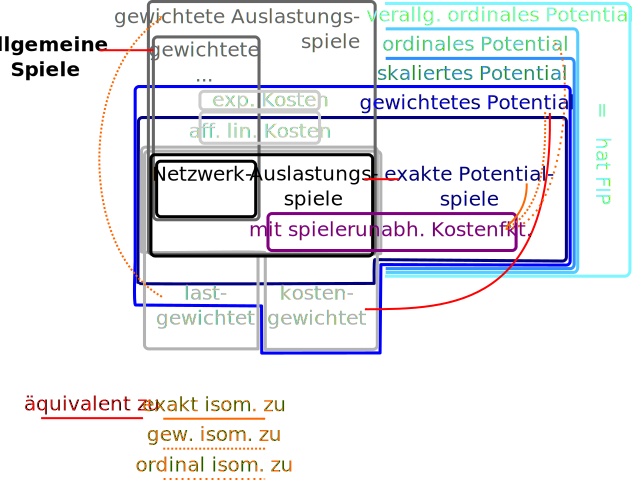
\includegraphics[width=.7\textwidth]{../Bilder/EulerDiagramm.pdf}
	\caption{Zusammenhänge zwischen den verschiedenen Spieleklassen für endliche Spiele}
\end{figure}

\phantomsection
\addcontentsline{toc}{section}{Ausblick}
\section*{Ausblick}

Wir haben nun also gesehen, wie (Iso-)Morphismen von Spielen genutzt werden können um Zusammenhänge zwischen Spielen zu formalisieren und zu verstehen welche Eigenschaften die zwei Spiele an den beiden Enden des Morphismus gemeinsam haben. Diese haben wir dann genutzt um verschiedene Aussagen über Potential- und Auslastungsspiele zu zeigen. Dabei ist es allerdings wichtig festzuhalten, dass die Verwendung von Morphismen hierbei niemals unumgänglich war, sondern die Aussagen immer auch ohne diesen Begriff hätten gezeigt werden können. 

Die Verwendung von Morphismen dient daher vor allem der einheitlicheren Beschreibung von Beziehungen zwischen Spielen, erleichtert die Strukturierung der Zusammenhänge, vereinfacht und verkürzt manche Aussagen und gibt möglicherweise auch neue Ideen für weitere Beziehungen. Auch ist es so besser möglich die verschieden starken Abstufungen von möglichen Beziehungen zu verstehen und etwa direkt zu sehen, welche Art von Beziehung man durch das Verknüpfen mehrerer solcher erhält.

Zunächst haben wir die Morphismenbegriffe dazu genutzt Potentiale durch passende Morphismen in Koordinationsspiele zu beschreiben. Dadurch hoffen wir einen neuen Blickwinkel auf Potentiale gewonnen zu haben. Ferner haben wir diesen Zusammenhang genutzt um einige Eigenschaften und Zusammenhänge der verschiedenen Potentialarten zu beweisen.

Sodann haben wir analoge Sätze zu dem von \citeauthor{MonShap} für gewichtete und skalierte Potentiale gesehen, haben Beste-Antwort-Isomorphismen und deren Verknüpfung dazu genutzt schnelle Konvergenz der Beste-Antwort-Dynamik für Matroidspiele zu zeigen und haben gesehen wie sich selbst nicht-anonyme Auslastungsspiele als gewöhnliche anonyme Auslastungsspiele darstellen lassen.

Gleichzeitig haben wir aber auch festgestellt, dass skalierte Auslastungsspiele bereits wieder eine zu große Klasse von Auslastungsspielen sind um vollständig in der Menge der Spielen mit skaliertem Potential enthalten sein zu können. Entsprechend unserer Suche nach einer passenden Klasse für Spiele mit gewichtetem Potential könnte man nun weiter nach einer passenderen Verallgemeinerung von kostengewichteten Auslastungsspielen suchen, die genau den skalierten Potentialspielen entspricht. 

Ein anderes Ziel könnte es sein andere Varianten zu finden, die noch allgemeineren Potentialspielen entsprechen. Vermutlich wird dies allerdings neue und aufwändigere Konstruktionen erfordern, da die Potentiale mit größerer Allgemeinheit immer weniger Information über das ursprüngliche Spiel enthalten. Ein skaliertes Potential etwa legt zusammen mit den Skalierungsfunktionen ein Spiel noch bis auf exakte Isomorphie eindeutig fest, ein ordinales Potential hingegen tut das nicht mehr (da hier zwar noch das Vorzeichen, aber keine Information mehr über die Größe der Änderungen eingeht).

Weitere Fragestelltungen könnten sein, welche Sätze man noch für unendliche Spiele verallgemeinern kann (v.a. \Cref{satz:JedesSpielGewAusl} und der zweite Teil von \Cref{satz:MondererShapley}) oder ob Konstruktionen in bereits existierenden Sätzen vereinfachen kann (etwa ob man analog zu \Cref{satz:GewAuslZuUngewAusl} gewichtete Auslastungsspiele mit affin exponentiellen Ressourcenkosten ohne den Umweg eines gewichteten Potentials direkt in isomorphe kostengewichtete Auslastungsspiele umwandeln kann). Und all diese Fragen lassen sich für kostenerhaltende Isomorphie (also Äquivalenz), aber - falls die entprechenden Aussagen nicht zugänglich oder sogar falsch sind - auch für die verschiedenen schwächeren Isomorphiebegriffe untersuchen.

\newpage
%\nocite{*}
\printbibliography

\end{document}
